%%
%% licence       kaneton licence
%%
%% project       kaneton
%%
%% file          /home/mycure/kaneton/view/exams/arch-mips/2006-partiel/2006-partiel.tex
%%
%% created       julien quintard   [fri dec  2 22:25:51 2005]
%% updated       julien quintard   [thu mar  2 19:06:00 2006]
%%

%
% template
%

%%
%% licence       kaneton licence
%%
%% project       kaneton
%%
%% file          /home/mycure/kaneton/view/templates/exam.tex
%%
%% created       julien quintard   [fri dec  2 22:20:57 2005]
%% updated       julien quintard   [mon feb 20 23:01:50 2006]
%%

%
% compile mode
%

%
% ---------- header -----------------------------------------------------------
%
% project       kaneton
%
% license       kaneton
%
% file          /home/mycure/kane...w/talk/presentations/kaneton/kaneton.tex
%
% created       julien quintard   [mon may 14 21:02:29 2007]
% updated       julien quintard   [sun feb  6 20:50:37 2011]
%

%
% ---------- setup ------------------------------------------------------------
%

%
% path
%

\def\path{../../..}

%
% template
%

%
% ---------- header -----------------------------------------------------------
%
% project       kaneton
%
% license       kaneton
%
% file          /home/mycure/kaneton/view/template/talk.tex
%
% created       julien quintard   [wed may 16 18:17:37 2007]
% updated       julien quintard   [fri may 23 19:28:10 2008]
%

%
% ---------- class ------------------------------------------------------------
%

\documentclass[8pt]{beamer}

%
% ---------- common -----------------------------------------------------------
%

\input{\path/package/opk/presentation.tex}


%
% title
%

\title{kaneton}

%
% document
%

\begin{document}

%
% title frame
%

\begin{frame}
  \titlepage
\end{frame}

%
% outline frame
%

\begin{frame}
  \frametitle{Outline}

  \tableofcontents
\end{frame}

%
% ---------- text -------------------------------------------------------------
%


%
% overview
%

\section{Overview}

% 1)

\begin{frame}
  \frametitle{Introduction}

  \term{kaneton} is an educational project intended for students to undertake
  in order to learn about operating system internals.
\end{frame}

% 2)

\begin{frame}
  \frametitle{History}

  \begin{itemize}
    \item[2004]
      \name{Julien Quintard} and \name{Jean-Pascal Billaud} decide
      to introduce an optional low-level programming course to first-year
      enginnering students, now known as \name{kastor};
    \item[2004]
      The course having been well received, \name{SRS - Syst\`emes, R\'eseaux,
      S\'ecurit\'e} students ask them to give such an introductory course the
      same year.
    \item[2005]
      The authorization is given to them to teach a kernel development course
      to \name{SRS} students, from January to October. They therefore decide
      to provide students with the design of a microkernel and let the students
      develop it from scratch, their way. \name{kaneton} is born.
    \item[2006]
      After \name{Jean-Pascal Billaud} fled to \name{VMWare}, \name{Julien
      Quintard} started developing a reference implementation and gave
      students this year a skeleton they had to complete. In addition,
      \name{Cedric Aubouy} and \name{Renaud Lienhart} joined the teaching
      team this year.

      \-

      Besides, the \name{LSE - Laboratoire Syst\`eme EPITA} joined the project
      by putting two students on the development of the \name{kaneton}
      research implementation. \name{Matthieu Bucchianeri} and \name{Renaud
      Voltz} thus joined the project.
  \end{itemize}
\end{frame}


% 3)

\begin{frame}
  \frametitle{History}

  \begin{itemize}
    \item[2007]
      This year, \name{Matthieu Bucchianeri} and \name{Renaud Voltz} took
      over the project for a year by lecturing the course and managing the
      project.

      \-

      \name{Julian Pidancet} and \name{Pierre Duteil} joined the project
      as part of the \name{LSE} but \name{Pierre Duteil} had to leave the
      project. Therefore, \name{Elie Bleton}, who was working at the
      \name{LRDE} before, joined the project.
    \item[2008]
      \name{Julian Pidancet} and \name{Elie Bleton} took over this year
      while \name{Laurent Lec} and \name{Nicolas Grandemange} joined as part
      of the \name{LSE}.

      \-

      At the end of this year, after problems with some students as well as
      conflicts with the \name{LSE}, \name{kaneton} maintainers decided not
      to work with the laboratory anymore.
    \item[2009]
      \name{EPITA} alumni were contacted and joined the educational project
      including \name{Francois Goudal}, \name{Benoit Marcot},
      \name{Enguerrand Raymond}, \name{Jean Guyader} but also
      \name{Fabien Le-Mentec}, an \name{EPITECH} alumnus.
  \end{itemize}
\end{frame}

% 4)

\begin{frame}
  \frametitle{Model}

  The project consists for students to fill in some missing parts of the
  kernel.

  \-

  However, note that, unlike \name{Tiger}, the missing parts will never
  be two lines long.

  \-

  Indeed, in \name{kaneton}, students are asked to implement a feature, say,
  providing memory management. Thus, students are free, in a certain way,
  to implement such a feature as they wish.

  \-

  Since the testing usually consists in verifying that the kernel is able
  to provide the functionality, students should be, most of the time, able
  to implement whatever algorithms \etc{} they wish.
\end{frame}

% 5)

\begin{frame}
  \frametitle{People}

  Let's present the people working on the educational project from where they
  studied to what they are now doing:

  \begin{itemize}
    \item
      \name{Francois Goudal};
    \item
      \name{Benoit Marcot};
    \item
      \name{Jean Guyader};
    \item
      \name{Baptiste Afsa}
    \item
      \name{Louis Vatier}; and
    \item
      \name{Julien Quintard}.
  \end{itemize}
\end{frame}

% 6)

\begin{frame}
  \frametitle{Project}

  \name{kaneton} is an important assignment of the \name{SRS}/\name{GISTR}
  curriculum and, as such, must be taken seriously.

  \-

  Especially, in the last years, \name{EPITA} decided to reduce the duration
  of the project to \term{three} months.

  \-

  As such, the other assignments imposed by the specializations in this
  period have been reduced so that students can focus on \name{kaneton}.
\end{frame}

%
% design
%

\section{Design}

% 1)

\begin{frame}
  \frametitle{Overview}

  The kaneton kernel is very different from the kernels you might be
  familiar with, especially the well-known \name{Windows}, \name{Linux},
  \name{BSD} and so forth.
\end{frame}

% 2)

\begin{frame}
  \frametitle{Microkernel}

  First, kaneton is a microkernel, making it modular from the design
  perspective as well as providing properties such as security.
\end{frame}

% 3)

\begin{frame}
  \frametitle{Distributed Computing}

  kaneton has been designed from the ground up for providing the operarting
  system advanced distributed computing features.
\end{frame}

% 4)

\begin{frame}
  \frametitle{Portability}

  kaneton has been designed with portability in mind, especially through
  a specific portability system that perfectly fits the kernel design.
\end{frame}

% 5)

\begin{frame}
  \frametitle{Organisation}

  Besides being a microkernel, kaneton is well organised in the inside,
  splitting functionalites into objects and managers.
\end{frame}

%
% stages
%

\section{Stages}

% 1)

\begin{frame}
  \frametitle{k0}

  The first project, named \term{k0}, consists for students to learn
  about low-level programming.

  \-

  This project comes with a lecture regarding the boot system as well
  as a practical session.

  \-

  \name{Francois Goudal} will be in charge of this stage which will last for
  a week.
\end{frame}

% 2)

\begin{frame}
  \frametitle{k1}

  \term{k1} consists for students to provide the kaneton microkernel the
  capacity to handle events.

  \-

  During this stage, a lecture on general kernel principles and a lecture on
  interrupts will be taught.

  \-

  \name{Julien Quintard} will be in charge of this stage which will last
  for a single week.

  \-

  Note that, starting with \name{k1}, the student snapshot will be used which
  provide students a development environment, making kernel development easier.
\end{frame}

% 3)

\begin{frame}
  \frametitle{k2}

  \term{k2} consists for students to provide the kaneton microkernel a
  memory management unit so that applications as well as the kernel itself
  can reserve, share \etc{} memory.

  \-

  During this stage, a lecture on portability as well as lectures on
  memory management will be taught.

  \-

  \name{Francois Goudal} will be in charge of this stage which will last
  for three weeks.
\end{frame}

% 4)

\begin{frame}
  \frametitle{k3}

  In \term{k3}, students will have to provide kaneton with execution contexts
  such that the kernel can execute multiple threads at the \textit{same} time.

  \-

  Lectures, during this stage, will discuss topics such as interrupts,
  concurrency, multi-processing, scheduling \etc{}

  \-

  \name{Benoit Marcot} will be in charge of this stage which will last for
  three weeks.
\end{frame}

% 5)

\begin{frame}
  \frametitle{Evaluation}

  For every stage, students will have the possibility to test their
  implementation by running, a limited number of times, the test suite used
  for evaluating their work.

  \-

  Besides, at the end of each stage, after submission, the kaneton test system
  will run the test suite and issue a mark according to the test results.

  \-

  Additionally, an exam will take place at the end of the semester to make
  sure that the notions tackled throughout the course are well understood
  by every student.
\end{frame}

%
% tools
%

\section{Tools}

% 1)

\begin{frame}
  \frametitle{Overview}

  The kaneton educational project relies on tools, sometimes developed
  internally.
\end{frame}

% 2)

\begin{frame}
  \frametitle{Web Site}

  The web site contains the documentation including design papers,
  the assignments \etc{} but also hosts the wiki which should be
  the starting point for every student seeking information.

  \-

  Noteworthy is that the wiki contains courses regarding the
  inline assembly, linking, pre-processing and so on. Students
  are invited to read them all as they will come handy when
  developing the kaneton stages.

  \-

  \name{Julien Quintard} should be contacted for requests regarding the
  web site and wiki.
\end{frame}

% 3)

\begin{frame}
  \frametitle{Snapshot}

  The student snapshot has been automatically generated from the current
  kaneton implementation.

  \-

  \name{Francois Goudal} is in charge of this process, hence should be
  contacted if you believe there is a mistake.
\end{frame}

% 4)

\begin{frame}
  \frametitle{Cheat}

  Every student's kaneton implementation will be tested to make sure that
  students did not cheat by relying on implementations by previous or
  current students.

  \-

  \name{Julien Quintard} is in charge of this tool.
\end{frame}

% 5)

\begin{frame}
  \frametitle{Test}

  Students' implementation will be tested in a real environment by applying
  a complete test suite; hence, validating the implementation's behaviour.

  \-

  \name{Jean Guyader} is responsible of this tool and should be contacted
  if necessary.
\end{frame}

%
% information
%

\section{Information}

% 1)

\begin{frame}
  \frametitle{Support}

  \begin{enumerate}
    \item
      \term{Website}

      \-

      You will find on \location{http://kaneton.opaak.org} documents regarding
      the project from the design to the implementation;
    \item
      \term{Wiki}

      \-

      The wiki \location{http://wiki.opaak.org} is the best way to get
      technical information as well as to help other students by adding
      and/or improving pages' contents;
    \item
      \term{Mailing-List}

      \-

      The kaneton educational students mailing-list
      \location{students@kaneton.opaak.org} will be used by teachers as
      an official means for communicating with students.

      \-

      Therefore, every student should subscribe to this mailing-list by sending
      an email to \location{students+subscribe@kaneton.opaak.org}.

      \-

      It is not allowed to post code on the mailing list, or give pointers to
      code in the snapshot that would provide obvious solution to somebody's
      question.
  \end{enumerate}
\end{frame}

% 2)

\begin{frame}
  \frametitle{Groups}

  Except for \name{k0} which is an individual project, the other projects
  from \name{k1} to \name{k3} are done in groups of \term{two} students.

  \-

  Every group is expected to send an email to
  \location{admin@opaak.org}.

  \-

  Note that we will use students' \name{EPITA} email addresses. As such,
  make sure that you check this email box.
\end{frame}

% 3)

\begin{frame}
  \frametitle{Reliance}

  As for \name{Tiger}, every stage depends on the previous one, except
  for \name{k0}.

  \-

  As such, test suites from the previous stages will also be used for both
  testing and marking.

  \-

  Students should therefore make sure to use their test permissions for making
  sure to fix the bugs of previous stages so that such bugs do not impact
  on the current stage results, hence mark.
\end{frame}

% 4)

\begin{frame}
  \frametitle{Machine}

  This year, the machine used by the kaneton educational project will consists
  of the \term{IBM-PC} platform coupled with the \term{IA-32} microprocessor
  architecture \ie{} the most common hardware system on the market.

  \-

  Although it is always best to test your implementation on a real machine,
  it takes time to reboot a real computer. You should therefore use an
  emulator such a \name{QEMU} or \name{Bochs} as they will enable you to
  test your kernel very quickly but they will also let you develop on
  a non-\name{IBM-PC}/\name{IA-32} machine such as a \name{Mac} for example.
\end{frame}

%
% conclusion
%

\section{Conclusion}

% 1)

\begin{frame}
  \frametitle{Concepts}

  Throughout the project, you will learn so many things from terminology,
  to how a computer boots, how the kernel controls the hardware and how it
  provides abstractions as basic as execution contexts.

  \-

  At the end of the project, you will definitely know that nothing is magic
  but purely logic and often actually very simple.
\end{frame}

% 2)

\begin{frame}
  \frametitle{Implementation}

  Although, starting the project by learning how to make a computer execute
  your code, you will end up, after three months, with a running kernel
  and operating system capable of executing programs, the whole on real
  hardware like the machine you have at home.
\end{frame}

% 3)

\begin{frame}
  \frametitle{Changes}

  Over the years, the project has greatly evolved, from a no-implementation
  project, to a reference-based project.

  \-

  However, being a project developed by volunteers willing to dedicate some
  time so that other students can learn, many things are missing and/or
  can be improved including the lectures but also the project implementation.

  \-

  In conclusion, keep in mind that the project exists only because of people
  willing to transfer their knowledge and please respect their effort.
\end{frame}

% 4)

\begin{frame}
  \frametitle{Fun}

  But most of all, kaneton should be about learning through fun!
\end{frame}

% 5)

\begin{frame}
  \frametitle{Reminder}

  Remember to perform the following tasks:

  \begin{itemize}
    \item
      Send an email to \location{admin@opaak.org} regarding the composition
      of your group, before \textbf{Wednesday 16th 2pm} or you will be put
      in a group by force;
    \item
      Subscribe to the students mailing-list
      \location{students@kaneton.opaak.org} by sending an email to
      \location{students+subscribe@kaneton.opaak.org};
    \item
      Watch closely the \name{Wiki} at \location{http://wiki.opaak.org} by
      subscribing the \name{RSS} feed for example;
    \item
      We advise SRS/GISTR lab roots to set up a \name{Xen}-based environment
      as testing on emulators only will become difficult over time;
    \item
      Students must have a ``rack'' containing a \name{POSIX}-compilant
      operating system for the \name{k0} practical session.
  \end{itemize}
\end{frame}

\end{document}


%
% class
%

\documentclass[10pt,a4wide]{article}

%
% packages
%

\usepackage[english]{babel}
\usepackage[T1]{fontenc}
\usepackage{a4wide}
\usepackage{graphicx}
\usepackage{fancyheadings}
\usepackage{multicol}
\usepackage{indentfirst}
\usepackage{color}
\usepackage{ifthen}
\usepackage{comment}
\usepackage{verbatim}
\usepackage{aeguill}

\pagestyle{fancy}

\setlength{\footrulewidth}{0.3pt}
\setlength{\parindent}{0.3cm}
\setlength{\parskip}{2ex plus 0.5ex minus 0.2ex}

%
% correction environment
%

\newenvironment{correction}%
   {
     \ifthenelse
	 {
	   \equal{\kaneton-latex}{subject}
	 }
	 {
	   \comment
	 }
	 {
	   \textbf{\color{red}{ ----- correction}}
	 }
   }%
   {
     \ifthenelse
	 {
	   \equal{\kaneton-latex}{subject}
	 }
	 {
	   \endcomment
	 }
	 {
	   \textbf{\color{red}{ ----- /correction}}
	 }
   }

%
% header
%

\rfoot{\scriptsize{Exam}}

\date{\scriptsize{\today}}


%
% header
%

\lhead{\scriptsize{2006}}

%
% title
%

\title{Examen d'Architecture MIPS}

%
% authors
%

\author{\small{Julien Quintard}}

%
% document
%

\begin{document}

%
% title
%

\maketitle

%
% --------- information -------------------------------------------------------
%

\begin{center}

\textbf{Documents Autoris\'es}

\textbf{Dur\'ee 3 heures}

\scriptsize{Une copie bien pr\'esent\'ee avec des sch\'emas propres et
	    lisibles sera toujours mieux not\'ee qu'une autre.}
\end{center}

%
% --------- text --------------------------------------------------------------
%

%
% assembleur
%

\section{Assembleur - 3 points}

Pour cet exercice nous consid\'erons un processeur pipeline comme celui
\'etudi\'e en cours. N\'eanmoins les d\'ependances entre instructions
n'existent pas pour cet exercice. Autrement dit, pour cet exercice,
le CPI est \'egal \`a 1 dans tous les cas.

Veuillez \'ecrire le code assembleur optimis\'e de la fonction
\textbf{strncpy()}.

Puis \'evaluer les performances de votre code assembleur pour une chaine
de caract\`eres de longueur N en calculant le nombre de cycles moyen
n\'ecessaire \`a l'ex\'ecution de votre fonction.

\begin{verbatim}
char*           strncpy(char* dst, const char* src, unsigned int size)
{
  int           i;

  for (i = 0; i < size && src[i]; i++)
    dst[i] = src[i];
  dst[i] = 0;

  return (dst);
}
\end{verbatim}

Un code assembleur avec une \'equivalence C en commentaire de fin de ligne
sera appr\'eci\'e.

\begin{correction}

  \begin{verbatim}
           Lw R5, 0(R29)                     ; dst
           Lw R6, 4(R29)                     ; src
           Lw R7, 8(R29)                     ; size

           Add R2, R0, R5                    ; R2: dst

           Add R16, R6, R7                   ; R16: pointeur fin de chaine

  Loop:    Lb R10, 0(R6)                     ; R10: *src

           Addiu R6, R6, 1                   ; src++

           Beq R10, R0, EndLoop              ; if (*src == '\0') goto EndLoop
           Sb R10, 0(R5)                     ; *dst = *src

           Bne R6, R16, Loop                 ; if (src != R16) goto Loop
           Addiu R5, R5, 1                   ; dst++

  EndLoop: Jr R31
           Nop
  \end{verbatim}

  \begin{verbatim}
    cycles = 5 + 6N + 4 + 2
           = 11 + 6N
  \end{verbatim}
\end{correction}

%
% vue simplifiee
%

\section{Vue simplifi\'ee - 4 points}

Dans cet exercice nous consid\'erons le microprocesseur pipeline \'etudi\'e
en cours incluant les d\'ependances entre instructions.

Vous pouvez si vous le d\'esirez retoucher votre code assembleur
pour qu'il soit plus performant vis-\`a-vis des d\'ependances entre
instructions.

Veuillez, pour la boucle principale de votre fonction \textbf{strncpy()},
d\'ecrire le pipeline en utilisant une vue simplifi\'ee.

Veuillez indiquer sur cette m\^eme vue simplifi\'ee les bypasses utilis\'es
entre les instructions d\'ependantes.

Puis \'evaluer les performances de votre boucle en calculant le CPI et CPI
utile.

\begin{correction}

  \begin{center}
    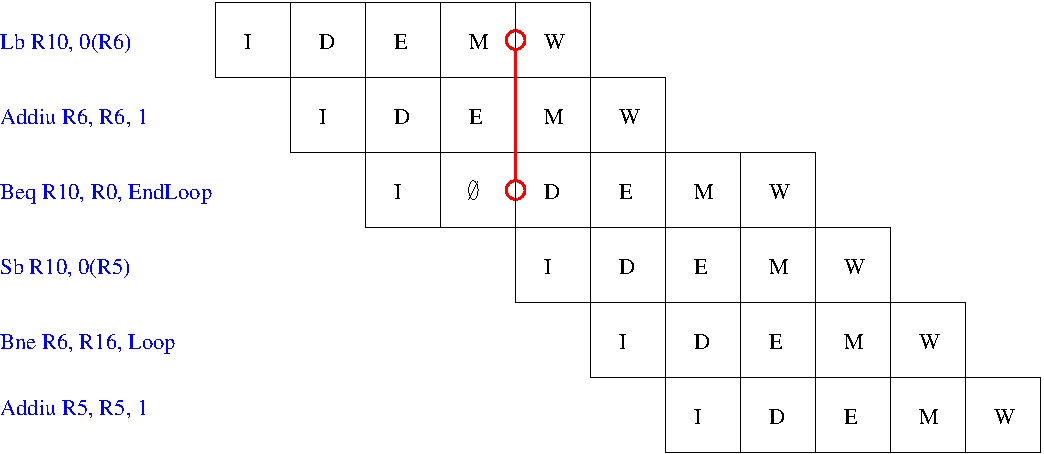
\includegraphics[scale=0.8]{figures/correction-vue-simplifiee.pdf}
  \end{center}

  \begin{verbatim}
    CPI = 7 / 6

    CPIu = 7 / 6
  \end{verbatim}

\end{correction}

%
% vue detaillee
%

\section{Vue D\'etaill\'ee - 5 points}

Veuillez d\'ecrire, via une vue d\'etaill\'ee, le pipeline pour l'instruction:

\textbf{Bltzal Rs, Label}: Branch if Less Than Zero And Link

Cette instruction, dans le cas du branchement, calcule l'adresse de
l'instruction suivante et sauvegarde \textit{l'adresse de l'instruction
courante + 4} dans le registre \textbf{R31} pour pouvoir continuer
l'ex\'ecution une fois la routine appell\'ee termin\'ee.

Pensez bien que votre pipeline doit g\'erer les deux cas: branchement
ou continuit\'e.

Un sch\'ema clair sera appr\'eci\'e surtout pour l'\'etage \textbf{DEC}.

\begin{correction}

  \begin{center}
    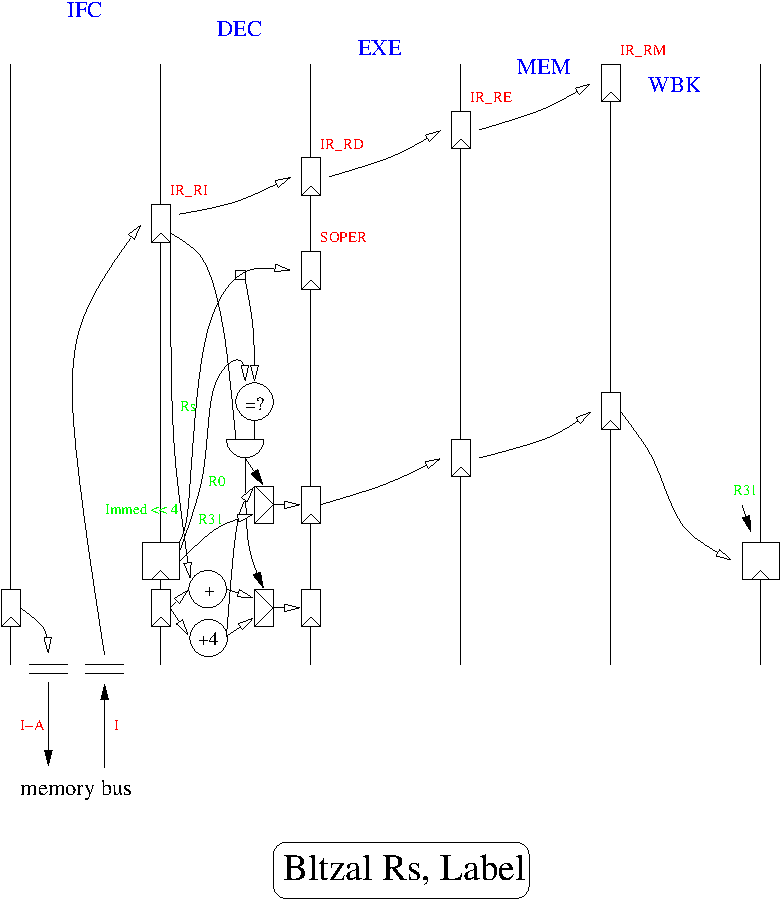
\includegraphics[scale=0.8]{figures/correction-vue-detaillee.pdf}
  \end{center}

\end{correction}

%
% questions de cours
%

\section{Questions de cours - 8 points}

\begin{enumerate}
  \item
    Quelles sont les principales diff\'erences entre la philosophie CISC
    et la philosophie RISC?

    \begin{correction}

      \textbf{CISC}

      \begin{itemize}
	\item
	  Jeu d'instructions complexe pour coller aux exigences des
	  langages de haut niveau.
	\item
	  Microprocesseur plus complexe car les instructions le sont.
      \end{itemize}

      \textbf{RISC}

      \begin{itemize}
	\item
	  Jeu d'instructions tr\`es simple.
	\item
	  Microprocesseur tr\`es simple.
	\item
	  Processeur essentiellement compos\'e de registres.
	\item
	  Les instructions registre-\`a-registre composent largement le
	  processeur. Les instructions d'acc\`es m\'emoire sont isol\'ees du
	  reste des instructions.
	\item
	  Les processeurs RISC ont la caract\'eristique d'ex\'ecuter chaque
	  instruction en un cycle.
      \end{itemize}

    \end{correction}
  \item
    Qu'est ce que la loi d'Amdhal?

    \begin{correction}

      La loi d'Amdhal est utilis\'ee par les concepteurs de microprocesseurs
      pour choisir correctement les instructions \`a inclure dans le
      jeu d'instructions du processeur.

      Cette loi dit que le gain r\'eel li\'e \`a l'inclusion d'une instruction
      est relatif \`a son temps d'ex\'ecution mais \'egalement au
      taux d'utilisation de cette m\^eme instruction.

    \end{correction}
  \item
    Veuillez d\'ecrire pr\'ecis\'ement quels types d'instructions sont
    encod\'ees dans chacun des formats \textbf{R}, \textbf{I} et \textbf{J}.

    \begin{correction}

      \textbf{Format R}

      \begin{itemize}
	\item
	  Les instructions registre-\`a-registre.
	\item
	  Les instructions de d\'ecalage de bits.
	\item
	  Les instructions qui peuvent \^etre cod\'es via ce format
	  car c'est ce format qui accepte le plus d'opcode.
      \end{itemize}

      \textbf{Format I}

      \begin{itemize}
	\item
	  Les instructions de branchement.
	\item
	  Les instructions qui ont besoin d'un imm\'ediat sur 16 bits.
      \end{itemize}

      \textbf{Format J}

      \begin{itemize}
	\item
	  L'unique instruction de saut \textbf{J}.
      \end{itemize}

    \end{correction}

    Consid\'erons l'ajout de l'instruction suivante:
    \textit{Chiche Rt, Rs, I}.

    Imaginons que cette instruction puisse se coder dans deux formats
    d'instruction diff\'erents, \textbf{R} et \textbf{I}.

    En tant que concepteur du processeur RISC MIPS R3000, quel
    format choisireriez-vous pour l'instruction \textit{Chiche} et pourquoi?

    \begin{correction}

      Puisque en tant que concepteurs nous avons le choix pour l'instruction
      \textit{Chiche} entre le format \textbf{R} et le format \textbf{I};
      nous allons sans aucun doute choisir le format \textbf{R} car celui-ci
      dispose d'un champ d'extension d'opcode.

      Pour \'economiser les opcodes il nous faut donc utiliser au maximum
      le format \textbf{R} d\`es que possible.

    \end{correction}
  \item
    D\'ecrire dans le d\'etail la gestion de l'instruction \textit{Andi}
    au niveau de la gestion de l'overflow.

    \begin{correction}

      L'instruction \textit{Andi Rt, Rs, Immed} effectue un \textit{ET logique}
      entre le registre source \textit{Rs} et l'imm\'ediat \textit{Immed}.

      Puis le r\'esultat sur 32-bit est rang\'e dans le registre destination
      \textit{Rt}.

      Pour pouvoir effectuer une op\'eration sur 32-bit les deux op\'erandes
      doivent \^etre sur 32-bit. Dans le cas d'une instruction avec
      un imm\'ediat, ce dernier est \'etendu \`a une valeur sur 32-bit.

      Puisque l'instruction \textit{Andi} est une op\'eration logique
      et non arithm\'etique, l'imm\'ediat sera consid\'er\'e comme
      un nombre non-sign\'e.

      De ce fait les 16 bits de poids forts seront tous simplement
      remplis de z\'eros et l'op\'eration pourra \^etre effectu\'ee
      correctement.

    \end{correction}
  \item
    R\'esumer de facon claire pourquoi, dans le cas d'un branchement,
    le calcul de l'adresse de l'instruction suivante n'est pas:

    \begin{verbatim}
      instruction address = branchment instruction address + immediate << 2
    \end{verbatim}

    \begin{correction}

      Lorsque l'\'etage \textbf{DEC} de l'instruction \textit{i} est
      ex\'ecut\'e, celui-ci ne connait pas l'adresse de sa propre instruction
      \textit{i} mais seulement celle de l'instruction \textit{i+1}.

      L'\'etage \textbf{DEC} pourrait alors soustraire \`a l'adresse de
      l'instruction \textit{i+1}, \textit{4} afin de retrouver l'adresse
      de l'instruction \textit{i} pr\'ec\'edente.

      Cette solution n'est pas une bonne id\'ee car l\'etage \textbf{DEC}
      est d\'ej\`a beaucoup trop compliqu\'e.

      Ainsi pour le raccourcir et donc \'equilibrer le pipeline, les
      concepteurs de MIPS ont pr\'ef\'er\'e simplifier l'\'etage en
      modifiant le calcul de l'adresse suivant dans le cas d'un branchement.

      Ainsi l'adresse suivante est calcul\'ee de la mani\`ere suivante:

      \begin{verbatim}
	instruction address = branchment instruction address + 4 +
                      immediate << 2
      \end{verbatim}

      ce qui est \'equivalent \`a:

      \begin{verbatim}
	instruction address = current instruction address + immediate << 2
      \end{verbatim}

    \end{correction}
  \item
    Pourquoi l'instruction \textit{Oriu} n'a pas de sens contrairement
    \`a l'instruction \textit{Addiu}.

    \begin{correction}

      Tout simplement parceque l'instruction \textit{Add} est une
      op\'eration arithm\'etique et peut donc s'utiliser avec des
      imm\'ediats sign\'es ou non.

      En revanche, l'instruction \textit{Oriu} n'a aucun sens puisque
      l'instruction \textit{Or} est une op\'eration logique. De ce fait
      l'imm\'ediat sera toujours consid\'er\'e comme non sign\'e.

      L'ajout du suffixe \textbf{u} n'a donc aucun sens pour cette instruction.

    \end{correction}
  \item
    Pourquoi l'instruction \textit{Nori} n'existe pas dans le jeu
    d'instructions.

    \begin{correction}

      Tout simplement parceque cette op\'eration peut \^etre effectu\'ee
      via d'autres instructions.

      Les concepteurs du processeur MIPS, en utilisant les MIXs et la
      loi d'Amdhal se sont rendus compte que cette instruction n'\'etait
      pas rentable et ne l'ont donc pas inclus dans le jeu d'instructions
      du microprocesseur.

      A noter que l'instruction \textit{Nori Rt, Rs, I} peut
      \^etre effectu\'ee via les instructions suivantes:

      \begin{verbatim}
	Addui Rd, R0, I
	Nor Rd, Rs, Rt
      \end{verbatim}

    \end{correction}

  \item
    Pourquoi est-ce que les pipelines modernes d\'ecoupent g\'en\'eralement
    les cycles d'acc\`es m\'emoire en plusieurs \'etages.

    \begin{correction}

      Le temps d'acc\`es de la m\'emoire a \'evolu\'e dans le temps mais
      beaucoup moins rapidement que celui des processeurs.

      Ainsi la diff\'erence de fr\'equence entre le microprocesseur et
      la m\'emoire s'est accrue.

      Pour limiter que cela n'affecte trop les performances des
      microprocesseurs modernes, les concepteurs d\'ecoupent les acc\`es
      m\'emoire en plusieurs \'etages.

    \end{correction}

\end{enumerate}

\end{document}
